\chapter{Приложение}
\label{ch:appendix}

\section{Приложение А. Теоретический вывод формул}


Эффектом Джоуля–Томсона называется изменение температуры газа при его адиабатическом дросселировании. Процесс дросселирования — это медленное протекание газа через дроссель под воздействием перепада давления. Дросселем можно назвать препятствие потоку газа в трубе в виде, например, пористой перегородки. Почти полностью закрытый и слегка пропускающий газ кран также можно считать дросселем. Пористой перегородкой может служить диск из керамики или пористого стекла. При дросселировании температура газа может как увеличиваться, так и уменьшаться. Очевидно, что такой процесс необратим. Рассмотрим его подробнее.\\
 
Получим теоретическое выражения для расчёта величины эффекта Джоуля–Томсона.

\begin{figure}[h!]
        \centering
        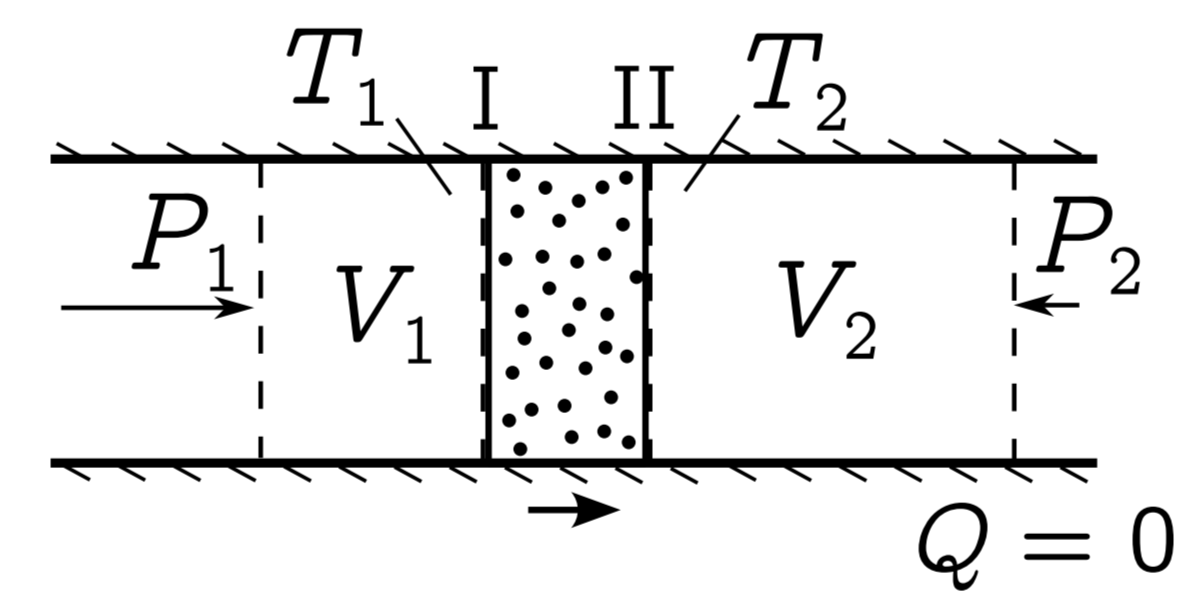
\includegraphics[scale=0.2]{img/216.png}
        \caption{
         \centering Принципиальная схема эффекта Джоуля–Томсона. Адиабатически изолированная труба с пористой перегородкой.
        }
 \end{figure} 




На рис. (1) изображена адиабатически изолированная труба с пористой перегородкой. Заметим, что разность давлений всегда $P_2 - P_1 = \Delta P < 0$, что говорит о существенной необратимости этого процесса. В силу его адиабатичности можно записать очевидное равенство:

\begin{equation}
Q = 0 = U_2 - U_1 + P_2V_2 - P_1V_1
\end{equation}

Здесь работа внешних сил равна $P_1V_1 < 0$, а $P_2V_2$ — работа самого газа, она положительна. Отсюда следует, что:

\begin{equation}
U_1 + P_1V_1 = U_2 + P_2V_2, \quad \text{т.е.} \quad I_1 = I_2.
\end{equation}

Значит, процесс дросселирования происходит при постоянстве энтальпии. 

В качестве характеристики процесса дросселирования введем величину, называемую коэффициентом Джоуля–Томсона:

\begin{equation}
\mu = \frac{\Delta T}{\Delta P},
\end{equation}

которая определяет эффект Джоуля–Томсона количественно. Поскольку для идеального газа энтальпия — однозначная функция температуры, то в связи с постоянством энтальпии для идеального газа $\Delta T = 0$, т.е. и $\mu = 0$. Конечно, для реального газа это уже далеко не так.

Рассмотрим так называемый дифференциальный эффект Джоуля–Томсона, т.е. эффект при малом перепаде давления на дросселе.

\begin{equation}
\mu = \left( \frac{\Delta T}{\Delta P} \right)_I \approx \left( \frac{\partial T}{\partial P} \right)_I.
\end{equation}

Запишем дифференциал энтальпии как функцию $T$ и $P$:

\begin{equation}
dI(T, P) = \left( \frac{\partial I}{\partial T} \right)_P dT + \left( \frac{\partial I}{\partial P} \right)_T dP = 0.
\end{equation}

Отсюда частная производная:

\begin{equation}
\left( \frac{\partial T}{\partial P} \right)_I = \mu = -\frac{\left( \frac{\partial I}{\partial P} \right)_T}{\left( \frac{\partial I}{\partial T} \right)_P} = -\frac{1}{C_P} \left( \frac{\partial I}{\partial P} \right)_T.
\end{equation}

Известна каноническая зависимость энтальпии от температуры и энтропии:

\begin{equation}
dI = T dS + V dP,
\end{equation}

Откуда при постоянной температуре искомая частная производная $\left( \frac{\partial I}{\partial P} \right)_T$ равна:

\begin{equation}
\left( \frac{\partial I}{\partial P} \right)_T = T \left( \frac{\partial S}{\partial P} \right)_T + V = -T \left( \frac{\partial V}{\partial T} \right)_P + V.
\end{equation}

Подставляя ее в (6), получим общее выражение для коэффициента Джоуля–Томсона при малом перепаде давления:

\begin{equation}
\mu \approx \left( \frac{\partial T}{\partial P} \right)_I = \frac{T \left( \frac{\partial V}{\partial T} \right)_P - V}{C_P}.
\end{equation}

Теперь из общего выражения (9) найдем коэффициент Джоуля–Томсона для газа Ван-дер-Ваальса. Для этого надо продифференцировать уравнение Ван-дер-Ваальса (  ) по температуре, считая давление $P$ постоянным:

\begin{equation}
-\frac{2a}{V^3} \left( \frac{\partial V}{\partial T} \right)_P (V - b) + \left( P + \frac{a}{V^2} \right) \left( \frac{\partial V}{\partial T} \right)_P = R.
\end{equation}

Искомая частная производная равна:

\begin{equation}
\left( \frac{\partial V}{\partial T} \right)_P = \frac{R}{P + \frac{a}{V^2} - \frac{2a(V - b)}{V^3}} = \frac{R(V - b)}{RT - \frac{2a(V - b)^2}{V^3}}.
\end{equation}

Для начала будем считать газ не очень плотным. Кроме того, пренебрежем величинами второго порядка относительно поправок $b$ и $a$. Тогда:

\begin{equation}
T \left( \frac{\partial V}{\partial T} \right)_P \approx \frac{V - b}{1 - \frac{2a}{RTV}} \approx (V - b) \left( 1 + \frac{2a}{RTV} \right) \approx V + \frac{2a}{RT} - b.
\end{equation}

Если подставить(9) в формулу для эффекта Джоуля–Томсона (12), получим окончательно:

\begin{equation}
\mu = \frac{\Delta T}{\Delta P} = \frac{\frac{2a}{RT} - b}{C_P}.
\end{equation}

Из этого выражения для $\mu$ сразу видно, что изменение температуры газа Ван-дер-Ваальса при необратимом расширении определяется поправками $a$ и $b$. При $a = b = 0$ $\mu = 0$. Кроме того, поправки $a$ и $b$ по-разному влияют на знак эффекта. Если силы взаимодействия между молекулами велики и преобладает поправка на давление, то можно считать $b = 0$, и тогда $\mu > 0$, т.е. $\Delta T < 0$ (газ охлаждается). Если силы взаимодействий малы и $a \to 0$, то преобладает поправка на объем $b$. В этом случае $\mu < 0$, и газ нагревается, т.е. $\Delta T > 0$ ($\Delta P < 0$).

\section{Приложение Б. Результаты измерений}

\begin{table}[h]
\centering
\begin{tabular}{|c|c|c|c|}
\hline
$t_0$, °C & $P$, бар & $\Delta V$, мкВ & $\Delta t$, °C \\ \hline
20.00 & 3.90 & -168 & -4.13 \\ \hline
20.00 & 3.50 & -150.00 & -3.69 \\ \hline
20.00 & 3.00 & -130.00 & -3.19 \\ \hline
20.00 & 2.50 & -106.00 & -2.60 \\ \hline
20.00 & 2.10 & -88.00 & -2.16 \\ \hline
20.00 & 1.70 & -66.00 & -1.62 \\ \hline
\end{tabular}
\caption{Экспериментальные данные, полученные при температуре термостата $t_0 = 20.00\,^\circ\text{C}$. Столбик $\Delta t$ получен из столбика $\Delta V$, зная зависимость чувствительности термопары от температуры термостата $t_0$.}
\end{table}

\begin{table}[h]
\centering
\begin{tabular}{|c|c|c|c|}
\hline
$t_0$, °C & $P$, бар & $\Delta V$, мкВ & $\Delta t$, °C \\ \hline
30.00 & 3.90 & -156.00 & -3.76 \\ \hline
30.00 & 3.60 & -141.00 & -3.40 \\ \hline
30.00 & 3.30 & -128.00 & -3.08 \\ \hline
30.00 & 2.90 & -115.00 & -2.77 \\ \hline
30.00 & 2.60 & -99.00 & -2.39 \\ \hline
30.00 & 2.20 & -86.00 & -2.07 \\ \hline
\end{tabular}
\caption{Экспериментальные данные, полученные при температуре термостата $t_0 = 30.00\,^\circ\text{C}$. Столбик $\Delta t$ получен из столбика $\Delta V$, зная зависимость чувствительности термопары от температуры термостата $t_0$.}
\end{table}

\begin{table}[h]
\centering
\begin{tabular}{|c|c|c|c|}
\hline
$t_0$, °C & $P$, бар & $\Delta V$, мкВ & $\Delta t$, °C \\ \hline
40.00 & 3.90 & -140.00 & -3.30 \\ \hline
40.00 & 3.50 & -124.00 & -2.92 \\ \hline
40.00 & 3.20 & -111.00 & -2.62 \\ \hline
40.00 & 2.80 & -95.00 & -2.24 \\ \hline
40.00 & 2.50 & -82.00 & -1.93 \\ \hline
\end{tabular}
\caption{Экспериментальные данные, полученные при температуре термостата $t_0 = 40.00\,^\circ\text{C}$. Столбик $\Delta t$ получен из столбика $\Delta V$, зная зависимость чувствительности термопары от температуры термостата $t_0$.}
\end{table}

\begin{table}[h]
\centering
\begin{tabular}{|c|c|c|c|}
\hline
$t_0$, °C & $P$, бар & $\Delta V$, мкВ & $\Delta t$, °C \\ \hline
50.00 & 3.90 & -128.00 & -2.96 \\ \hline
50.00 & 3.50 & -111.00 & -2.57 \\ \hline
50.00 & 3.00 & -96.00 & -2.22 \\ \hline
50.00 & 2.60 & -79.00 & -1.83 \\ \hline
50.00 & 2.00 & -54.00 & -1.25 \\ \hline
\end{tabular}
\caption{Экспериментальные данные, полученные при температуре термостата $t_0 = 50.00\,^\circ\text{C}$. Столбик $\Delta t$ получен из столбика $\Delta V$, зная зависимость чувствительности термопары от температуры термостата $t_0$.}
\end{table}